\documentclass[11pt,a4paper]{article}
\usepackage[margin=2.2cm]{geometry}
\usepackage[T1]{fontenc}
\usepackage{lmodern,microtype,amsmath,amssymb,graphicx,booktabs,tabularx,array,enumitem,float}
\usepackage[table]{xcolor}
\usepackage{caption}
\usepackage{tikz}
\usetikzlibrary{arrows.meta,positioning}
\usepackage[hidelinks]{hyperref}
\graphicspath{{../results/figures/}}
\captionsetup{font=small,labelfont=bf}
\setlength{\parskip}{3pt}

\title{\vspace{-1.4cm}\textbf{Who Made This Voice?}\\[3pt]
\large Training-free attribution of audio deepfakes, studied with speech-processing tools\\[6pt]
\normalsize AI553 Speech and Audio Processing --- Course Project Report}
\author{Saaransh Garg (2024AIB1011) \quad \textcolor{red}{[Partner name] ([Roll no.])}\\
\small Indian Institute of Technology Ropar}
\date{November 2026}

\begin{document}
\maketitle

\begin{abstract}
\noindent Detecting that speech is synthetic is no longer enough: forensic use needs to know
\emph{which} system produced it, and to say ``unknown'' when the generator is new. We study
TADA~\cite{stan2025tada}, a training-free method that embeds each clip with a frozen
self-supervised model (w2v-BERT~2.0) and labels it with $k$-nearest neighbours. Using 9{,}800
clips from 19 generators of ASVspoof~2019 LA, we compare it with features from the course
(MFCC, LFCC, LPC cepstra, GMMs). TADA attributes 13 generators with 97.6\,\% accuracy, and
97.0\,\% on speakers never seen before, against 72.2\,\% for MFCC. A sub-band analysis shows
that the classical fingerprint sits mostly in the 4--8\,kHz band, which the mel scale
compresses. The kNN distance detects unseen generators with 96.6\,\% AUROC. Two
``unseen'' systems that re-use known algorithms are mapped to their true counterparts
(100\,\% and 98\,\%). Under simulated channels (8\,kHz resampling, $\mu$-law, MP3) the
self-supervised features keep 91--95\,\% accuracy while the classical features collapse,
but additive noise breaks all of them.
\end{abstract}

% =====================================================================================
\section{Introduction}
Modern text-to-speech (TTS) and voice-conversion (VC) systems can imitate a voice from
seconds of audio. Telling real from fake is a well-studied problem; \emph{attribution}
(source tracing) asks the harder forensic question of \emph{which generator} made a clip.
Because new generators appear constantly, a useful system must also recognise when a clip
comes from a generator it has never seen (\emph{open set}).

TADA~\cite{stan2025tada} (Interspeech 2025) proposes a strikingly simple solution: average
an early hidden layer of a frozen pre-trained speech model over time, and classify with
$k$-NN. Nothing is trained. We study \emph{why} it works and \emph{where it breaks}, using
course tools as instruments:
\begin{enumerate}[label=\textbf{RQ\arabic*},leftmargin=3em,itemsep=0pt]
  \item How do course features (MFCC, LFCC, LPCC, GMM) compare, and which frequency band
        carries the fingerprint?
  \item Does the method recognise the \emph{generator} or just the \emph{speaker}?
  \item Can the kNN distance flag unseen generators?
  \item How robust is attribution to channel effects from the course: sampling,
        quantisation, filtering, noise and perceptual coding?
\end{enumerate}

% =====================================================================================
\section{Background: why generators leave fingerprints}
A TTS system is a chain: text $\rightarrow$ \emph{acoustic model} $\rightarrow$ acoustic
features $\rightarrow$ \emph{waveform generator} (vocoder) $\rightarrow x[n]$; VC replaces the
text front-end with analysis of a source speaker. The ASVspoof~2019 generators~\cite{wang2020asvspoof}
cover the vocoder families met in the course:
\emph{source-filter} vocoders (WORLD, STRAIGHT, Vocaine: a pulse/noise excitation filtered
by a spectral envelope), \emph{LPC filtering} (A06/A19), \emph{Griffin--Lim} phase
reconstruction from the STFT magnitude (A11)~\cite{griffin1984signal}, neural
autoregressive vocoders (WaveNet, WaveRNN)~\cite{oord2016wavenet}, and unit-selection
concatenation of real recordings (A04/A16). Each leaves consistent traces: band limits,
over-regular excitation, phase incoherence, joins. These traces are what attribution
exploits. Fig.~\ref{fig:spectro} shows examples.

\begin{figure}[t]
\centering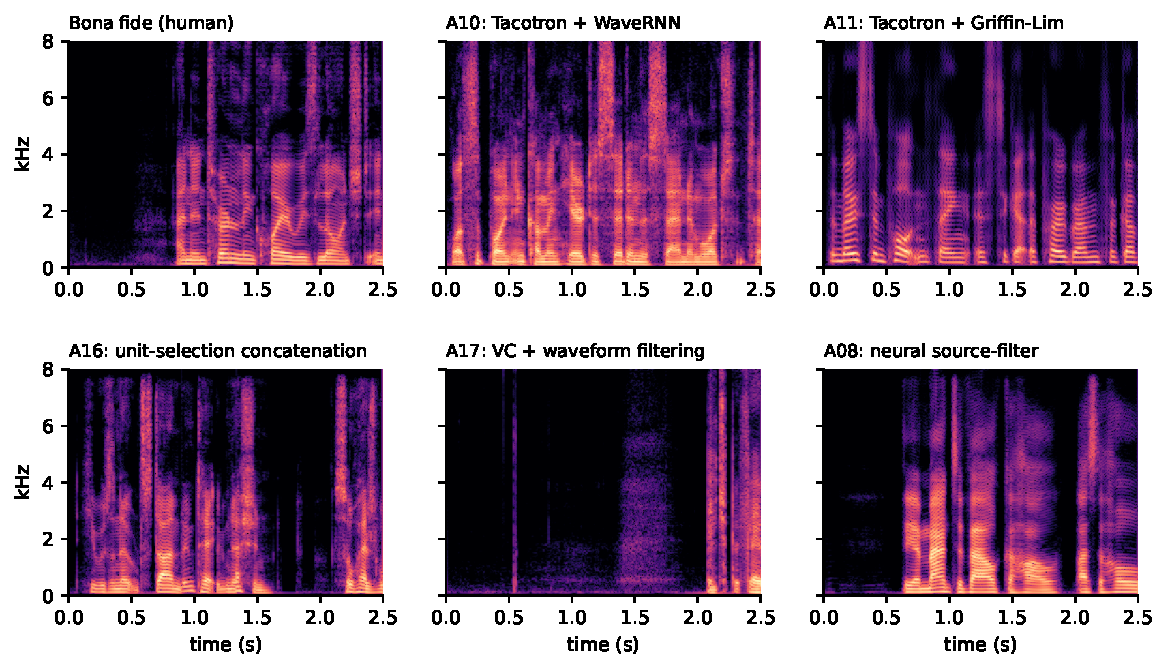
\includegraphics[width=\linewidth]{spectrograms}
\caption{Spectrograms (0--8\,kHz) of a human clip and five generators. The differences in
high-frequency texture, harmonic sharpness and noise floor are the ``fingerprints''.}
\label{fig:spectro}
\end{figure}

\paragraph{Course features.} All follow short-time analysis: pre-emphasis
$y[n]=x[n]-0.97x[n-1]$, 25\,ms frames every 10\,ms, a window, and $|\mathrm{DFT}|^2$.
\textbf{MFCC}~\cite{davis1980mfcc} applies 40 mel-spaced triangular filters
($\mathrm{mel}(f)=2595\log_{10}(1+f/700)$), a log and a DCT, keeping 13 coefficients.
\textbf{LFCC} uses 20 \emph{linearly} spaced filters, so 4--8\,kHz is resolved as finely as
0--4\,kHz; it is the ASVspoof baseline front-end~\cite{sahidullah2015features}.
\textbf{LPCC} fits a 16th-order all-pole model $H(z)=G/A(z)$ per frame by solving the
Yule--Walker equations with Levinson--Durbin~\cite{makhoul1975lpc}, converts $A(z)$ to cepstral
coefficients and appends the log residual energy (the \emph{source}). All three add
$\Delta,\Delta\Delta$; the mean and standard deviation over frames give one vector per clip
(78, 120 and 34 dimensions).

\paragraph{w2v-BERT 2.0 and TADA.} w2v-BERT~2.0~\cite{barrault2023seamless,chung2021w2vbert}
is a 600\,M-parameter Conformer encoder (24 blocks) pre-trained without labels on 4.5\,M hours
of speech. Its input is an 80-band log-mel filterbank. TADA averages the output of block~4
over time, giving a 1024-d vector, and classifies it with Euclidean $k$-NN ($k=21$). The mean
distance to the $k$ nearest support vectors is the out-of-domain (OOD) score.

% =====================================================================================
\section{Data and its challenges}
We use ASVspoof~2019 LA~\cite{wang2020asvspoof}, whose three partitions have disjoint
speakers: \emph{train} and \emph{dev} contain generators A01--A06, and \emph{eval} contains
A07--A19. A16 and A19 are, by design, the same algorithms as A04 and A06. The full corpus is
7.6\,GB, so our download script reads only the metadata columns of the parquet files, plans
a speaker-balanced sample, and fetches only the needed 100-row blocks (292 of 1{,}216). This
gives 400 clips per class for train (A01--A06 + bona fide, 20 speakers) and eval
(A07--A19 + bona fide, 67 speakers), and 200 per class for dev (20 speakers): 9{,}800 clips,
8.9\,h, about 3.2\,s each.

\textbf{Challenges.} (i)~\emph{Speaker confound:} every generator speaks with the same 67
eval speakers, so a random split puts the same voice in support and test. (ii)~\emph{Hidden
duplicates:} A16/A19 are ``new'' labels for old algorithms. (iii)~\emph{Partition shift:} OOD
tests mix new generators with new speakers. (iv)~Real channels (telephone, compression,
noise) alter exactly the fine spectral detail that carries the fingerprint.

% =====================================================================================
\section{Method}
\begin{figure}[h]
\centering
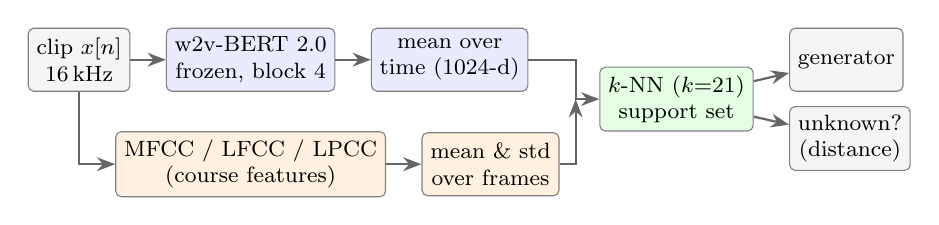
\begin{tikzpicture}[node distance=3.5mm and 4.5mm,
  b/.style={draw=black!50,rounded corners=2pt,fill=#1,align=center,font=\footnotesize,minimum height=8mm,inner sep=3pt},
  b/.default=black!4, a/.style={-Stealth,black!60,thick}]
  \node[b] (x) {clip $x[n]$\\16\,kHz};
  \node[b=blue!8,right=of x] (s) {w2v-BERT 2.0\\frozen, block 4};
  \node[b=blue!8,right=of s] (p) {mean over\\time (1024-d)};
  \node[b=orange!12,below=5mm of s] (c) {MFCC / LFCC / LPCC\\(course features)};
  \node[b=orange!12,right=of c] (st) {mean \& std\\over frames};
  \node[b=green!10,right=9mm of p,yshift=-5mm] (k) {$k$-NN ($k$=21)\\support set};
  \node[b,right=of k,yshift=5mm] (l) {generator};
  \node[b,right=of k,yshift=-5mm] (o) {unknown?\\(distance)};
  \draw[a] (x)--(s); \draw[a] (s)--(p); \draw[a] (x)|-(c); \draw[a] (c)--(st);
  \draw[a] (p)-|([xshift=-3mm]k.west)--(k.west); \draw[a] (st)-|([xshift=-3mm]k.west);
  \draw[a] (k)--(l); \draw[a] (k)--(o);
\end{tikzpicture}
\caption{Pipeline. Both branches produce one vector per clip; the same training-free $k$-NN
does attribution and unseen-generator detection.}
\label{fig:pipe}
\end{figure}

\textbf{Classifiers.} The main classifier is $k$-NN with $k=21$ (TADA). Classical vectors are
z-scored with support-set statistics first. As a classical statistical baseline from the
course, we fit one 32-component diagonal GMM per generator on \emph{frame-level} LFCCs (EM)
and pick the generator with the highest mean log-likelihood. w2v-BERT runs in fp16 on a
laptop RTX~2050 (checked against fp32: cosine $\ge 0.9998$ in every layer).

\textbf{Protocols.} \emph{Attribution:} the 13 eval generators (5{,}200 clips), five
stratified 80:20 splits, and five \emph{speaker-disjoint} splits that hold out 20\,\% of the
speakers. \emph{Open set:} the support set is A01--A06 from train; the known test set is
A01--A06 from dev (new speakers); the unknown set is A07--A19. We report AUROC and the
equal error rate (EER), the threshold at which false alarms equal misses. \emph{Robustness:}
the support set stays clean, and the 1{,}040 test clips of split~0 pass through each channel of
Table~\ref{tab:robust} before feature extraction.

% =====================================================================================
\section{Results}

\subsection{Attribution: SSL vs.\ course features (RQ1, RQ2)}
\begin{table}[t]
\centering\small
\caption{Attribution accuracy (\%) over the 13 ASVspoof 2019 eval generators (kNN, $k=21$; mean $\pm$ std over 5 splits). ``Unseen speakers'': test speakers never appear in the support set.}
\label{tab:attr}
\begin{tabular}{lcc}
\toprule
Feature & Random split & Unseen speakers \\
\midrule
MFCC & 72.2 $\pm$ 1.1 & 67.6 $\pm$ 3.5 \\
LFCC & 76.4 $\pm$ 1.0 & 71.4 $\pm$ 1.6 \\
LFCC 0--4 kHz & 73.9 $\pm$ 1.4 & 70.7 $\pm$ 1.8 \\
LFCC 4--8 kHz & 84.3 $\pm$ 0.3 & 78.7 $\pm$ 1.8 \\
LPCC & 71.2 $\pm$ 1.0 & 62.9 $\pm$ 2.5 \\
LFCC frames + GMM (32 comp.) & 96.6 $\pm$ 0.4 & -- \\
\textbf{w2v-BERT layer 4 (TADA)} & 97.6 $\pm$ 0.4 & 97.0 $\pm$ 1.0 \\
\bottomrule
\end{tabular}
\end{table}

\begin{figure}[t]
\centering
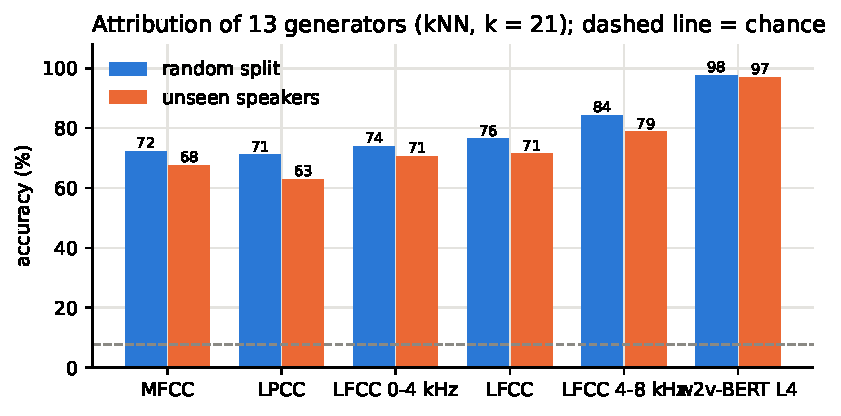
\includegraphics[width=0.49\linewidth]{feature_comparison}\hfill
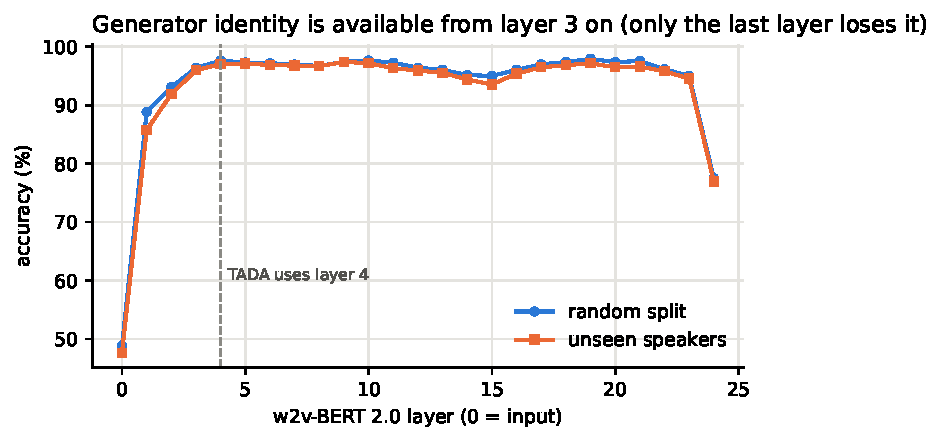
\includegraphics[width=0.49\linewidth]{layer_sweep}
\caption{Left: accuracy per feature (chance = 7.7\,\%). Right: accuracy of every w2v-BERT
layer; layer~0 is the input projection.}
\label{fig:attr}
\end{figure}

Table~\ref{tab:attr} and Fig.~\ref{fig:attr} give the main answer. The frozen w2v-BERT
features reach \textbf{97.6\,\%}, against 72.2\,\% for MFCC and 76.4\,\% for LFCC. Three
course-related observations:
\begin{itemize}[itemsep=1pt]
  \item \textbf{The mel scale hides the fingerprint.} LFCC beats MFCC, and LFCC computed on
        the \emph{4--8\,kHz band alone} (84.3\,\%) beats both the full band and the
        0--4\,kHz band (73.9\,\%). The mel scale is designed for human hearing and spends
        few filters on high frequencies, but that is where vocoder artefacts (band limits,
        noise floors, phase errors) are most visible.
  \item \textbf{Frame statistics matter.} A GMM on frame-level LFCCs reaches 96.6\,\%,
        close to w2v-BERT, because it models the whole distribution of frames rather than
        only their mean and standard deviation. Unlike $k$-NN, it must be \emph{trained}
        (EM) whenever a generator is added.
  \item \textbf{Layers.} The input projection (layer~0) gives only 48.8\,\%. Accuracy reaches
        96--98\,\% by layer~3 and stays there until the last layer (77.5\,\%), where the
        model has become most abstract. TADA's layer~4 is the cheapest layer at peak
        accuracy: only 4 of 24 blocks are needed.
\end{itemize}

\subsection{Generator or speaker? (RQ2)}
With speaker-disjoint splits, w2v-BERT loses only 0.6 points (97.0\,\%), whereas MFCC loses
4.6 and LPCC 8.3 (Table~\ref{tab:attr}). The SSL features therefore capture the generator
rather than the voice; the classical features lean partly on the speaker. The confusion
matrix (Appendix, Fig.~\ref{fig:conf}) shows that the SSL errors concentrate on A10
(WaveRNN; 89\,\% recall). LFCC confuses pairs that share an acoustic model but differ in
the vocoder (A14 STRAIGHT $\rightarrow$ A15 WaveNet, 24\,\%), and w2v-BERT separates them
perfectly.

\subsection{Unseen generators (RQ3)}
\begin{table}[t]
\centering\small
\caption{Detecting unseen generators (\%). Known: A01--A06; unknown: the 11 genuinely new eval generators. A16/A19 re-use the A04/A06 algorithms, so an AUROC near 50 means they are correctly seen as known.}
\label{tab:ood}
\begin{tabular}{lcccc}
\toprule
Feature & AUROC & EER & A16 AUROC & A19 AUROC \\
\midrule
MFCC & 77.9 & 29.6 & 73 & 35 \\
LFCC & 74.3 & 34.2 & 71 & 28 \\
w2v-BERT layer 4 (TADA) & 96.6 & 9.3 & 78 & 73 \\
\bottomrule
\end{tabular}
\end{table}

\begin{figure}[t]
\centering
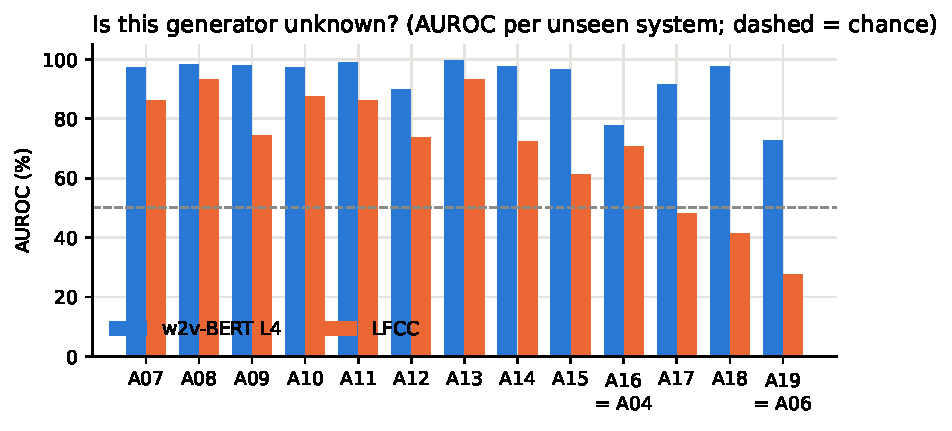
\includegraphics[width=0.56\linewidth]{ood_per_system}\hfill
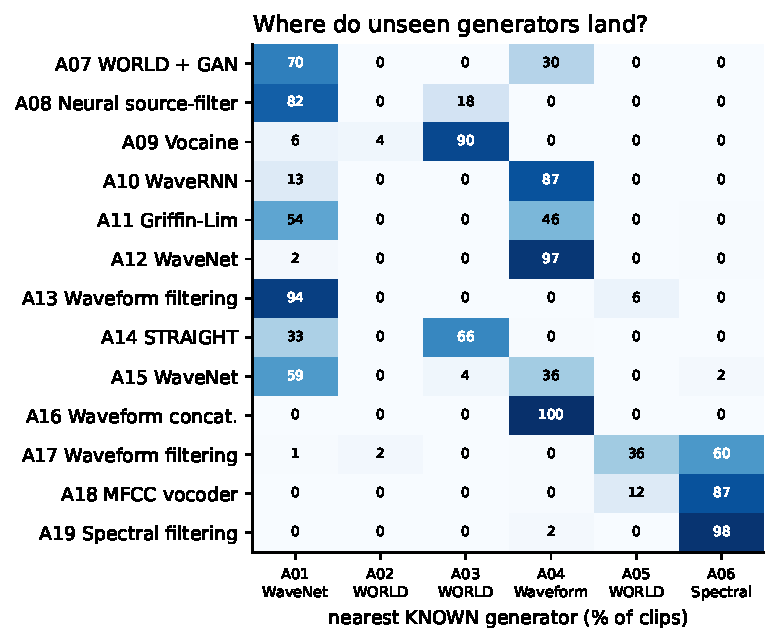
\includegraphics[width=0.40\linewidth]{ood_forced_choice}
\caption{Left: AUROC for detecting each eval generator as unknown. Right: when forced to
choose a known generator, A16 lands on A04 (100\,\%) and A19 on A06 (98\,\%), which are their true algorithms.}
\label{fig:ood}
\end{figure}

The $k$-NN distance on w2v-BERT features separates known from genuinely new generators with
\textbf{96.6\,\% AUROC} (EER 9.3\,\%), far ahead of MFCC (77.9\,\%) and LFCC (74.3\,\%); see
Table~\ref{tab:ood}. On the known generators themselves, closed-set accuracy across the
train$\rightarrow$dev speaker change is 99.9\,\%. The built-in control behaves as hoped
(Fig.~\ref{fig:ood}). A16 and A19 are the least ``novel'' systems (AUROC 78 and 73, against
90--100 for the others), and the nearest known generator for 100\,\% of A16 and 98\,\% of A19
clips is A04 and A06 respectively, their true algorithms. The residual separation (AUROC above
50) reflects the partition shift: different speakers and recording sessions.

\subsection{Robustness to channel effects (RQ4)}
\begin{table}[t]
\centering\small
\caption{Attribution accuracy (\%) when test audio passes through a channel the (clean) support set never saw. 13 generators, 1040 test clips.}
\label{tab:robust}
\begin{tabular}{lcccc}
\toprule
Test channel & MFCC & LFCC & LPCC & w2v-BERT L4 \\
\midrule
Clean & 73.2 & 76.8 & 71.0 & 98.0 \\
8 kHz resample & 51.5 & 49.1 & 14.1 & 92.5 \\
Uniform 8-bit & 32.7 & 20.6 & 20.2 & 83.6 \\
$\mu$-law 8-bit & 52.5 & 42.1 & 30.4 & 95.4 \\
Noise 20 dB & 7.8 & 8.1 & 8.5 & 51.6 \\
Noise 10 dB & 5.7 & 7.7 & 7.4 & 29.2 \\
Low-pass 4 kHz & 51.2 & 43.1 & 11.8 & 95.5 \\
High-pass 4 kHz & 8.2 & 14.6 & 8.6 & 7.7 \\
MP3 32 kbps & 46.3 & 19.2 & 38.1 & 90.7 \\
\bottomrule
\end{tabular}
\end{table}

\begin{figure}[t]
\centering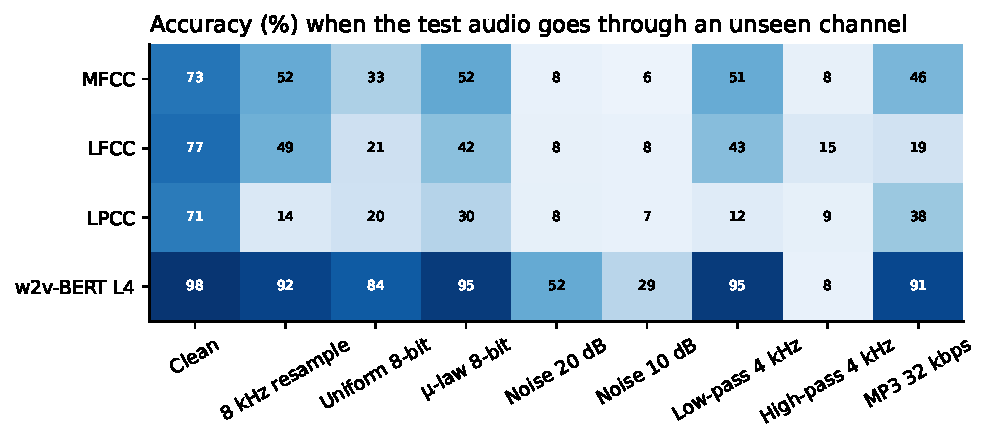
\includegraphics[width=0.85\linewidth]{robustness}
\caption{Accuracy (\%) when the test audio passes through a channel never seen in the support set.}
\label{fig:robust}
\end{figure}

Every degradation is a course topic (Table~\ref{tab:robust}, Fig.~\ref{fig:robust}). The
classical features collapse under almost any channel. LPCC drops from 71\,\% to 14\,\% with
8\,kHz resampling, since the all-pole fit changes when the 4--8\,kHz band disappears.
w2v-BERT is far more robust. It keeps 92\,\% after 8\,kHz resampling (sampling theorem: the
anti-aliasing filter removes everything above 4\,kHz), 95\,\% after a 4\,kHz low-pass and
91\,\% after MP3 at 32\,kbit/s. \textbf{$\mu$-law companding (95\,\%) beats uniform 8-bit
quantisation (84\,\%)}, exactly as the SQNR argument from the course predicts: companding
keeps quiet segments accurate. Two conditions break every feature: additive noise (52\,\% at
20\,dB, 29\,\% at 10\,dB) masks the low-level detail that the fingerprint lives in, and
keeping only 4--8\,kHz (high-pass) leaves w2v-BERT at chance, because its mel input front-end
relies on the low band.

% =====================================================================================
\section{Discussion and limitations}
\textbf{What the method matches.} Three pieces of evidence point to the generator rather than
the speaker or the dataset. Accuracy barely changes on unseen speakers; generators that share
an acoustic model but use different vocoders are separated; and re-used algorithms (A16/A19)
are mapped to their originals. \textbf{Training-free is a real advantage.} The GMM nearly
matches $k$-NN on clean data, but every new generator requires refitting, whereas $k$-NN
just stores new vectors.

\textbf{Limitations.} (i)~We use a 9{,}800-clip subset of a single corpus. (ii)~Attribution
assumes the input is fake: in our demo a human clip lands next to A19, a voice-conversion
system that filters real speech, unless bona fide speech is added to the support set as its
own class. (iii)~Open-set detection does not transfer easily across corpora: clips from 2025
TTS systems (MLAAD) received low vote agreement (8--13 of 21) but were not always flagged,
in line with TADA's own cross-dataset findings. (iv)~Robustness was tested only in the
mismatched setting; adding degraded audio to the support set would help, especially against
noise.

% =====================================================================================
\section{Connection to the course}
\begin{table}[H]
\centering\small
\begin{tabularx}{\linewidth}{@{}>{\raggedright\arraybackslash}p{4.2cm}X@{}}
\toprule
\textbf{Course topic} & \textbf{Where it is used} \\
\midrule
Sampling theorem, narrow/wideband speech & 8\,kHz resampling channel; 0--4 vs.\ 4--8\,kHz sub-band LFCC \\
Quantisation, SQNR, $\mu$-law & Uniform vs.\ $\mu$-law 8-bit channels; unit test of $6.02b+1.76$\,dB \\
LTI filtering, pre-emphasis & Butterworth low/high-pass channels; pre-emphasis in every front-end \\
DFT/STFT, windows, spectrograms & All features; spectrogram analysis of generators (Fig.~\ref{fig:spectro}) \\
Source-filter model, LPC, autocorrelation & LPCC via Levinson--Durbin; vocoder families explained as source-filter systems \\
Mel scale, cepstrum, MFCC, $\Delta$ & MFCC vs.\ LFCC: perceptual warping discards the forensic band \\
GMM & Per-generator GMM baseline on frame-level LFCC \\
Template matching / distances & $k$-NN attribution and distance-based open-set detection \\
Perceptual coding (hearing) & MP3 channel \\
\bottomrule
\end{tabularx}
\end{table}

\section{Conclusion}
A frozen self-supervised model plus $k$-NN attributes 13 real generators at 97.6\,\%, holds up
on unseen speakers and most channels, and flags new generators with 96.6\,\% AUROC, all
without training. Course tools explain much of \emph{why}: the fingerprint lies largely in
spectral detail that the mel scale compresses and that noise masks. Future work: a bona fide
gate in front of attribution, support sets built from degraded audio, and evaluation on
modern TTS corpora.

\bibliographystyle{ieeetr}
\bibliography{refs}

\appendix
\section{Additional figures}
\begin{figure}[H]
\centering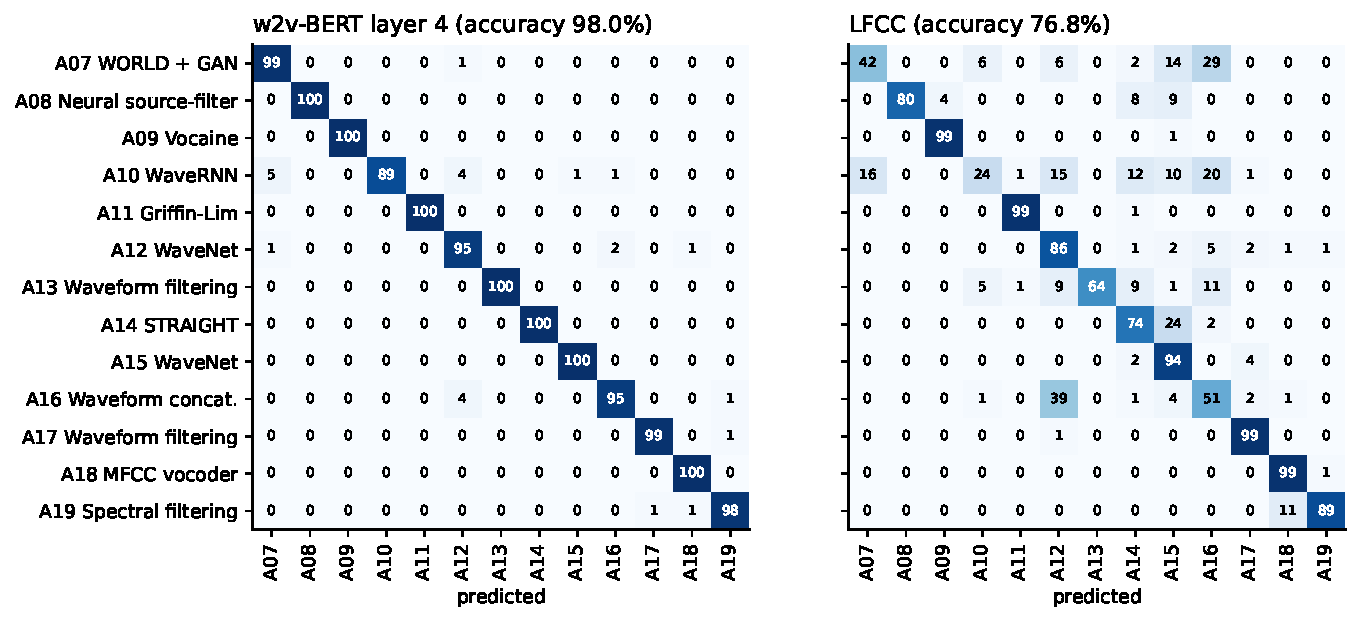
\includegraphics[width=\linewidth]{confusion}
\caption{Confusion matrices (split 0, \% of each true generator).}
\label{fig:conf}
\end{figure}
\begin{figure}[H]
\centering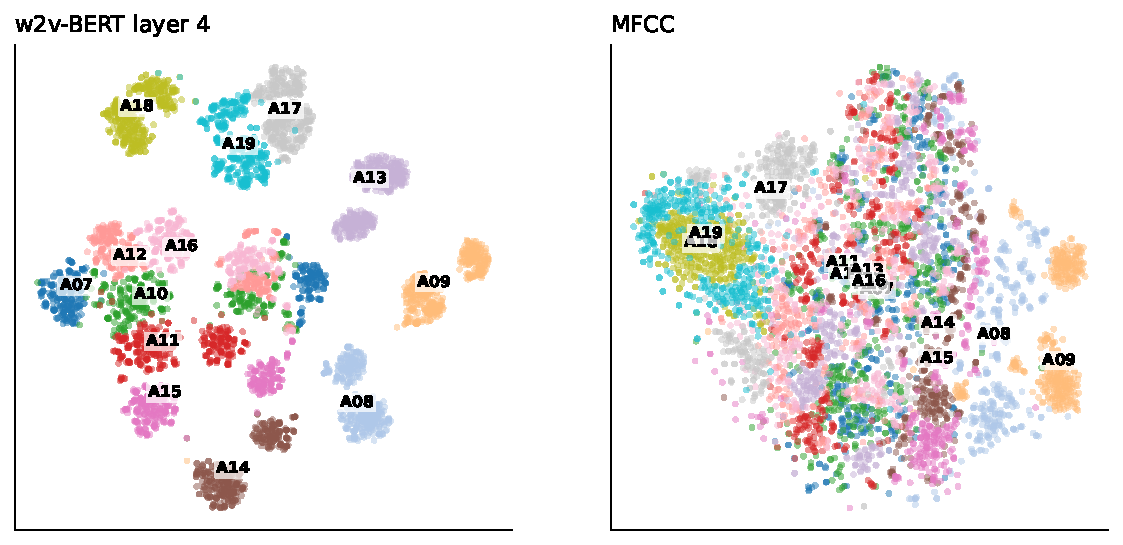
\includegraphics[width=\linewidth]{tsne}
\caption{t-SNE of the 13 generators: w2v-BERT forms clean clusters; MFCC overlaps heavily.}
\end{figure}

\section{Reproducing the results}
\texttt{pip install -r requirements.txt}, then \texttt{bash run\_all.sh}. This downloads the
data, extracts features (about 15\,min on a 4\,GB GPU), runs \texttt{scripts/3\_experiments.py}
and \texttt{scripts/4\_figures.py}, and writes every number to \texttt{results/results.json}.
Seeds are fixed. \texttt{python demo.py} runs the live demo.

\section{Contributions}
\textcolor{red}{[Team to fill in: who did what.]}

\section{Disclosure of AI-tool use}
As required by the course, we disclose that we used \textbf{Claude Code} (Anthropic; model
Claude Opus~5.5) as a coding and writing assistant. It helped to check facts in the TADA and
ASVspoof~2019 papers, wrote most of the code and figures, ran the experiments on our laptop,
and drafted this report and the slides. The team chose the research questions, reviewed and
ran all code, and is responsible for the content. All numbers come from the scripts in the
repository (\texttt{results/results.json}). Details are in \texttt{AI\_DISCLOSURE.md}.

\end{document}
